\section{The Road Network}
\label{sec:theroadnetwork}

The road network determines the road setup and how can cars move in it. The road network definition is based on the ideas implemented in OpenStreetMap \cite{OSM}. The goal of the OpenStreetMap project is to provide a free geographic data, and allow users to contribute for the improvement of said maps.

\subsection{A quick introduction to OpenStreetMap}

The information here given is mostly taken from the OpenStreetMap Wiki page, more detailed information can be found there.

OpenStreetMap is based on three fundamental elements, nodes, ways and relations.

\begin{description}
  \item[Nodes] A node is an individual point on a map. Associated to each point is a set of GPS coordinates, latitude and longitude, and a unique indentifier, an id. Two or more nodes can be connected together to form complex shapes. This is done making use of ways. Figure \ref{fig:osm_nodes} shows a group of nodes.
  \item[Ways] A way is a line of nodes. This line is formed by connecting the nodes belonging to the way through straight segments. Several different ways can be formed with the same set of nodes, the order of the nodes in the way is then essential for it's correct definition. Ways can close on themselves, forming closed ways. Closed ways can be useful to define areas or regions. Figure \ref{fig:osm_way} shows an example of a way, notice that the way has a defined direction, if the nodes were ordered in reverse, the direction would be the opposite.
  \item[Relations]A relation is used to described more complex concepts that might involve multiple ways. That said a relation can be thought of as a grouping of ways, just like a way is a grouping of nodes. A relation is composed by it's members, and their roles in the relation.
\end{description}

\begin{figure}[h!]
  \centering
    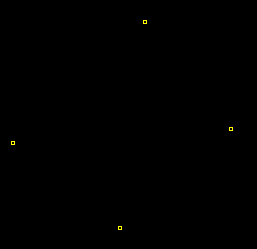
\includegraphics[width=0.5\textwidth]{osm_nodes}
    \caption{Visualisation of four nodes (visualisation using JOSM) \label{fig:osm_nodes} }
\end{figure}

\begin{figure}[h!]
    \centering
    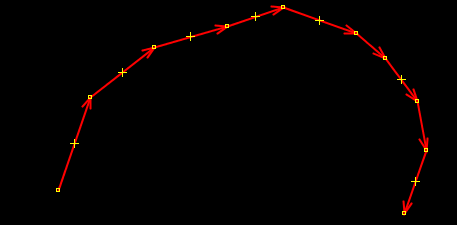
\includegraphics[width=0.5\textwidth]{osm_way}
    \caption{Visualisation of a way made up of ten nodes (visualisation using JOSM) \label{fig:osm_way} }
\end{figure}

Furthermore each of these elements can have tags. A tag is simply extra information that can be added to every element. A tag is defined by its name and value.

Making use of the simple concepts explained previously it is possible to define very complex maps.

\subsection{Adapting OpenStreetMap to the SML World}

In order to define our SML World road network, we will make use of the OpenStreetMap elements, however some additional concepts/conventions have to be defined.

\subsubsection{Introduction to Lanelets}

Lanelets are the main concept used when defining the SML World road network. A lanelet is a particular case of an OSM Relation and it defines a road lane. Any road lane is defined by its limits (left and right lane markings). Road lanes also need a direction to be defined (unless they are bi-directional).

The creation of a lanelet is as follows:

\begin{enumerate}
\item Create the way (and respective nodes) corresponding to the left lane markings
\item Create the way (and respective nodes) corresponding to the right lane markings
\item Create a relation, and add as members the previous ways, with the respective roles, left\_lane\_marking and right\_lane\_marking
\end{enumerate}

The direction of the lanelet is defined by the direction of the right\_lane\_marking way. Whatever the direction of left\_lane\_marking might be, the direction of the lanelet will be the same as the direction of the right\_lane\_marking way.

Let us imagine we wish to define the road shown in figure \ref{fig:road_to_define}. These road is section is composed of two lanes, and as such we will need two lanelets to define this road. First we need to define the ways, that correspond to the left and right lane markings. In order to create these ways, we need first to add the corresponding nodes. Figure \ref{fig:road_to_define_with_nodes} shows the nodes that need to be created in order to define the ways corresponding to the lane markings. Once these nodes are added, we simple create the respective ways, as shown in figure \ref{fig:road_to_define_with_ways}. The orange and pink ways, will be the right\_lane\_marking of each lanelet, whilst the blue way will be the left\_lane\_marking of both lanelets. Note that the direction of the right lane marking will always define the direction of the lanelet, and as such it is important that this way is correctly oriented. It might be confusing that the same way, and the same direction, is used for the left\_lane\_marking of both lanelets, but this will not be a problem, as we simply use the left\_lane\_marking of a lanelet to know where a lane boundary is, not its direction.

\begin{figure}[h!]
  \centering
    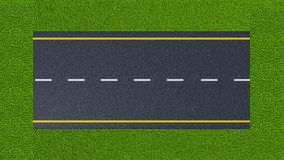
\includegraphics[width=0.5\textwidth]{road_original}
    \caption{The road section that we wish to define \label{fig:road_to_define} }
\end{figure}

\begin{figure}[h!]
    \centering
    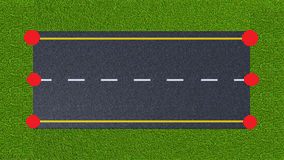
\includegraphics[width=0.5\textwidth]{road_with_nodes}
    \caption{Road section overlayed with necessary nodes \label{fig:road_to_define_with_nodes} }
\end{figure}

\begin{figure}[h!]
    \centering
    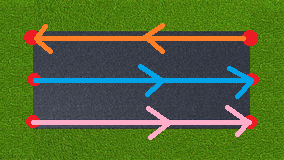
\includegraphics[width=0.5\textwidth]{road_with_ways}
    \caption{Road section overlayed with necessary ways \label{fig:road_to_define_with_ways} }
\end{figure}

\subsubsection{Defining a Road Network using Lanelets}

A road network can be created making use of several lanelets. First however we need to define the concept of Lanelet Adjacency.

\textbf{Lanelet Adjacency} Two lanelets, $L_a$ and $L_b$, are said to be adjacent if the first node of the right\_lane\_marking of $L_b$ is the same as the last node of the right\_lane\_marking of $L_a$.

When two lanelets are adjacent, we know that a car can travel from one lanelet to the other. The importance of the lanelet adjacency stems from the need of needing to generate realistic and law-conforming paths for the cars to drive on.

Figure \ref{fig:intersection_original} shows a three way intersection with the corresponding lanelets that lead into it. The lanelets are shown in a very simplified way, by a straigh segment in the middle of each lanelet. With each segment there is an associated arrow, indicating the direction of the lanelet.

\begin{figure}[h!]
    \centering
    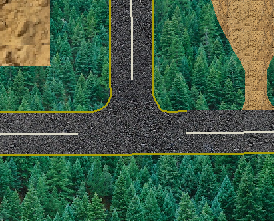
\includegraphics[width=0.5\textwidth]{intersection_original}
    \caption{A three way road intersection \label{fig:intersection_original} }
\end{figure}

The lanelets that describe the possible movements in this intersection are shown in figures \ref{fig:intersection_paths_group_1}, \ref{fig:intersection_paths_group_2} and \ref{fig:intersection_paths_group_3}.

\begin{figure}
    \centering
    \begin{subfigure}[b]{0.3\textwidth}
        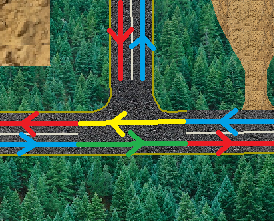
\includegraphics[width=\textwidth]{intersection_paths_group_1}
        \caption{Lanelets connecting left and right sections}
        \label{fig:intersection_paths_group_1}
    \end{subfigure}
    ~ %add desired spacing between images, e. g. ~, \quad, \qquad, \hfill etc. 
      %(or a blank line to force the subfigure onto a new line)
    \begin{subfigure}[b]{0.3\textwidth}
        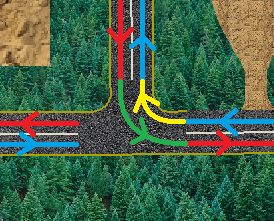
\includegraphics[width=\textwidth]{intersection_paths_group_2}
        \caption{Lanelets connecting top and right sections}
        \label{fig:intersection_paths_group_2}
    \end{subfigure}
    ~ %add desired spacing between images, e. g. ~, \quad, \qquad, \hfill etc. 
    %(or a blank line to force the subfigure onto a new line)
    \begin{subfigure}[b]{0.3\textwidth}
        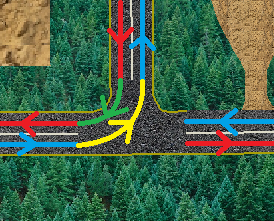
\includegraphics[width=\textwidth]{intersection_paths_group_3}
        \caption{Lanelets connecting top and left sections}
        \label{fig:intersection_paths_group_3}
    \end{subfigure}
    \caption{All the possible lanelets in a three way intersection}
\end{figure}

When all the lanelets of the intersection are put together, we create a functional piece of road network, with well defined car paths. Remember that a car can only travel between adjacent lanelets, and as such the road intersection does not allow for illegal movements, such as moving to a lane with a different direction.

Using this concept of lanelets and lanelet adjacency we can create a big variety of road networks with well defined rules of traffic flow. This is of extreme importance as we will see in the following sections.

MAYBE DO A LIST OF ADJACENCIES.

\subsection{Creating a Road Network}

Once the concepts of the road network are understood, we can start creating one. For this purpose we will use JOSM.

\subsubsection{JOSM}

JOSM\cite{JOSM} is an OpenStreetMap editor. This editor provides a GUI to edit OpenStreetMap files/maps. We will make use of it to create a file that will define our road network. Figure \ref{fig:josm_sml} shows a snapshot of a JOSM program instance running.

\begin{figure}[h!]
    \centering
    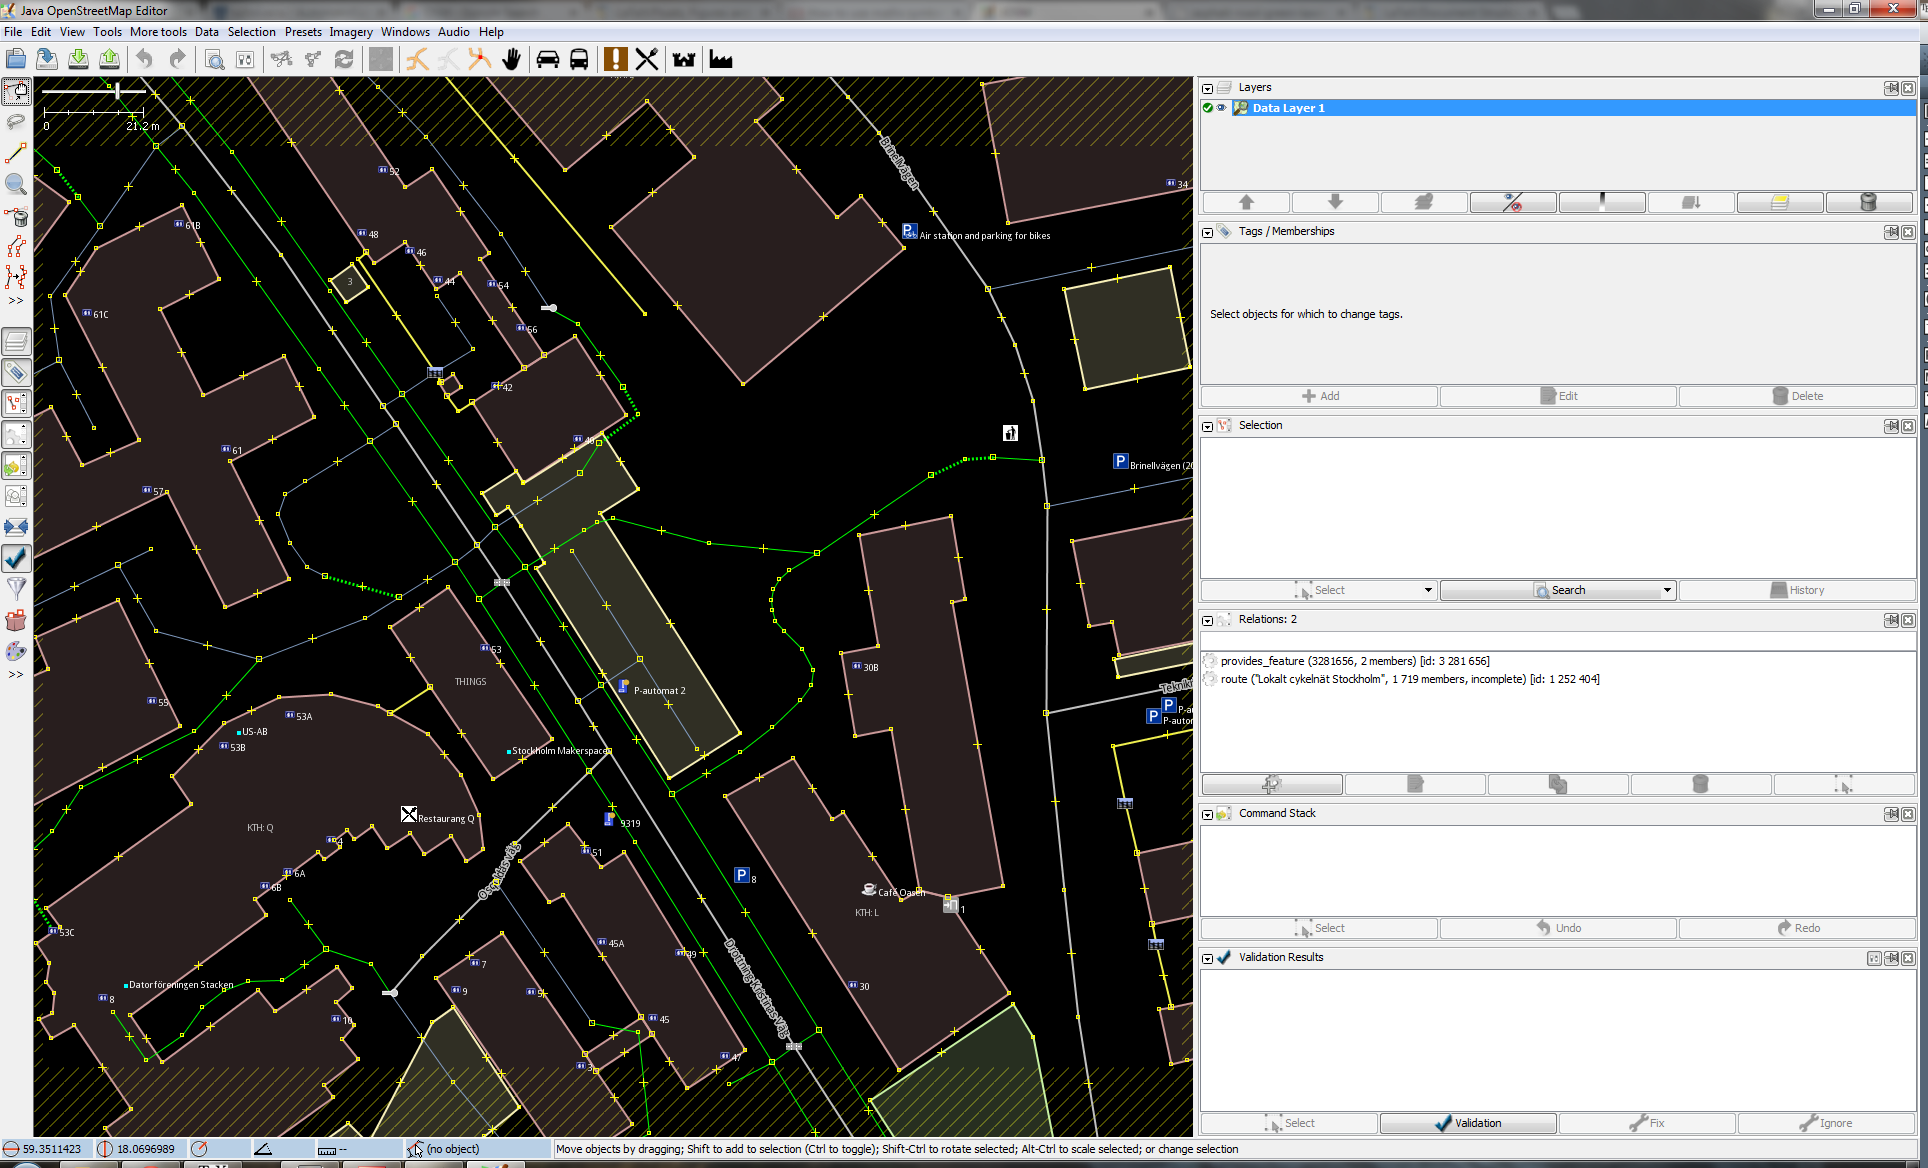
\includegraphics[width=0.75\textwidth]{JOSM_SML}
    \caption{An overview of the SML and surroudings OpenStreetMap map making use of JOSM \label{fig:josm_sml} }
\end{figure}

Here it will not be explained how to use JOSM, only how to build our road network making use of it. To understand how to work with JOSM refer to the guide available online.

\subsubsection{Creating a Lanelet}

Before creating a lanelet, we need to create the ways corresponding to its left and right road markings. Lets start by creating the right road marking. To do so we simply create a way with the orientation that we wish our lanelet to have.

We could now use the same procedure to create the left road marking, however we are going to make use of the parallel tool to remove the ammount of work that placing the nodes requires. Besides being more efficient the parallel tool also guarantes that the new lane marking is parallel and in the same shape as the original lane marking, which should happen in every road.

An important detail is that the lanelet road marking ways need to have the same ammount of nodes, otherwise they cannot be processed by the SML World. The parallel tool complies with this requirement.

Once both ways are defined, we simply need to create our relation, which will represent a lanelet. Simply create a new relation, and the tag "type"="lanelet" and associate as members "right\_road\_marking" and "left\_road\_marking" the respective ways. The lanelet is now defined. 

\subsubsection{Connecting Lanelets}

To connect lanelets, i.e., to make them adjacent we simply need to make sure that they have the same orientation, and that the first node of right way in one of the lanelets corresponds to the last node in the other lanelet.


\subsubsection{Saving the Road Network File}

When the road network is complete, its corresponding information must be saved. JOSM allows saving the road network in several different file types, however we are interested in saving the file with the \textit{.xml} extension, meaning that we will have a simple to read XML file that can be easily used for future purposes.

If we wish to edit a previously save map, we simply need to open the corresponding \textit{.xml} file, edit it and save it again.

\subsubsection{General Tips}

Using the parallel tool is often a good practice, due to the reasons already stated.

JOSM provides several tool, however that are some extra tools that can be added through the use of plugins. One of these tools is Circle Arc, which allows the user to draw circle arcs with relative ease.


\subsubsection{List of Existing Road Networks OSM Files}

Some Road Networks were already made for previous usages. Their filenames and an explanation of their purposes will be given here.

\begin{description}

\item[HighwaySML.xml] This is the road network of a circular Highway with three lanes, all in the counter clockwise direction. This road network was used by the Summer Students of 2015, and it served to show possible solutions to the GCDC scenarios of platoons merging and emergency vehicle. The highway dimensions were fitted so that they allow for real live demonstrations using the scaled trucks. This road network can be altered to larger dimensions for simulation purposes.
\item[MiningEnvironmentSML.xml] This defined the road network used in the May 2015 IQMatic demonstration at Scania. It is composed of several roads and intersections, and it special environments for the scaled trucks to perform Autonomous Driving manoeuvres, like reverse driving and path planning. This map is not supported by the current SML World version, but can be useful in the creation process of new maps.
\item[SodertaljeResidentialArea.xml] This road network was based on a real residential road network. Defining road networks based on real existing ones can be useful to show and evaluate the performance of the autonomous driving system in realistic scenarios. This map is not supported by the current SML World version.
\item[RoadTemplates.xml] This file contains some useful and complex road network elements, like three and four way intersections. They can be easily copied for the creation of new maps.
\end{description}

